\documentclass[11pt]{amsart}

\usepackage{a4wide}
\usepackage{paralist}
\usepackage{url}
\usepackage{nopageno}
\usepackage{graphicx}
\usepackage{bbm}

\newcommand{\cA}{\mathcal{A}}
\newcommand{\cS}{\mathcal{S}}

\begin{document}
\begin{center}
\textbf{\sffamily
   Discrete and Algorithmic Geometry }

\medskip
   Julian Pfeifle,
   UPC, 2013 \mbox{}
\end{center}

\bigskip

\begin{center}
  \textbf{\sffamily Sheet 2}

\bigskip
 due on Monday, November 18, 2013

\end{center}

\bigskip
\bigskip
\bigskip

\section*{Reading}

\begin{enumerate}
\setlength{\itemsep}{2ex}
%\item Read Lectures 0,1,2 from Ziegler's \emph{Lectures on Polytopes}.

%\item Read Sections 5.1, 5.2, 5.3 from Matou\v sek's \emph{Lectures on
%    Discrete Geometry}.
\item
\end{enumerate}

\bigskip
\bigskip
\section*{Writing}

\begin{enumerate}
\item Show that all induced cycles of length $3$, $4$ and $5$ in the graph of a simple $d$-polytope~$P$ are graphs of $2$-faces of $P$.
Conclude that the Petersen graph is not the graph of any polytope (of any dimension).

(\emph{Hint for $5$-cycles:} First show this for $d=3$, then prove
that any $5$-cycle in a simple polytope is contained in some $3$-face,
and use that a face of a simple polytope is simple.)

\item Let $n\in\mathbbm{N}$ be an integer and $S$ denote a subset of
  $\{1,2,\dots,\lfloor\frac{n}{2}\rfloor\}$.  
  The \emph{circulant graph} $\Gamma_n(S)$ is the graph whose vertex set is $\mathbbm{Z}_n$, and whose edge set is the set of pairs of vertices whose difference lies in $S\cup (-S)$. 

The following figure collects all connected circulant graphs on up to $8$~vertices. Determine the \emph{polytopality range} of each of these graphs, i.e., the set of integers~$d$ such that the graph in question is the graph of a $d$-dimensional polytope.

\bigskip
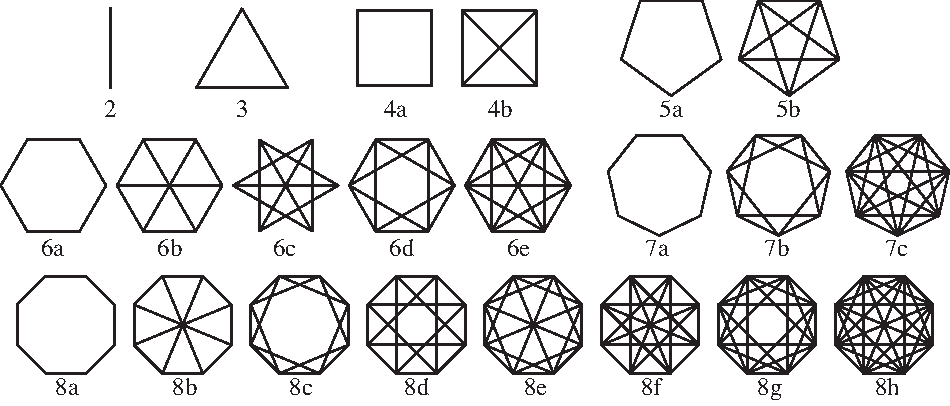
\includegraphics[width=\linewidth]{circulant}
\end{enumerate}

\bigskip
\bigskip
\section*{Software}

\begin{enumerate}
\setlength{\itemsep}{2ex}
\item
\end{enumerate}

\end{document}
